\section{Road Intersection Density}

% how density could indicate formal
% the estimated accuracy?
% add picture to explain
% how intersections found in images
% ^ theoretical background
%

As a novel approach for the distinction between formal and informal regions, we
propose the density of intersections as a metric. This is on the belief that
area's with a dense road network, resulting in many intersections, are well
developed, thus indicating a formal region. Informal regions, on the other
hand, would be characterized by a dip in the density of intersections.  

This metric is constructed using road extraction techniques. The area of road
extraction has developed over the years, starting from 1970. A straightforward
method for road extraction is the use of edge detection. Because roads have
distinct properties due to material, design and function, the appearance of
roads are often quite in contrast to the environment. For example, on satellite
images, the homogenious black color and the regular straight lines make
roads easily identifiable from the suroundings for the human eye. Edge
detection uses the sharp contrast between a road and the roadside to identify
the road.


\subsection{Intersection extraction methods}

Besides tradional image processing methods, another promising approach in the
detection of road networks from satellite images are Neural Networks
\cite{mangala2011extraction} \cite{mokhtarzade2007road}. A study from 2017 was
able to extract both the road network together with buildings with high
accuracy using a Convolutional Neural Network \cite{alshehhi2017simultaneous}.

We used a seperate implementation of the convolutional neural network since the
research paper did not include the software used \cite{airs}. This
implementation includes a set of images, that could be used for the training
and validation of the neural network \cite{MnihThesis}. After the training of
the network on the provided images, was used to extract the roads from our own
satellite images.  Unfortunately, the mask of the road network was erroneous as
it did not represent the road network in the provided image. The suspected
cause of this failure is the difference in the training data to our satellite
imagery data.

To illustrate the difference, the trainingset contained satellite images
obtained from partly rural area's of the state of Massachusetts in the United
States while the data used in our research is from Bangalore in India which is
mostly urban.  As a result, the geographical features and the road systems are
quite different in the two area's. This could cause the network not to
recognize the roads in the images from Bangalore. The difference in resolutions
of the two image sets could be another cause. The images of Massachusets were
of a lower resolution than the images of Bangalore which could have hindered
the neural network in the correct classification of the roads, although this is
ungrounded speculation.

\subsection{Hough Transform}
% TODO: cite Otsu
%
As a alternative to neural network, conventional image processes were used. The
image is subjected to a number of operations that will extract the road network
from the image. The first operation is the transformation of the RGB satellite
image to grayscale values. This is done in preparation for Otsu's method for 
threshold, which effectively separates buildings from roads. The resulting
image, although quite crude, is a mask of the road network in the satellite image.
Because are roads are straight lines on satellite image data, these straight
lines can be captured using a Hough transform. Hough transform is able to
detect straight lines in images. Once we have the mathematical definition of
the lines, the location of the intersection can be located.

\begin{figure}
\begin{tabular}{cc}
  \subfloat{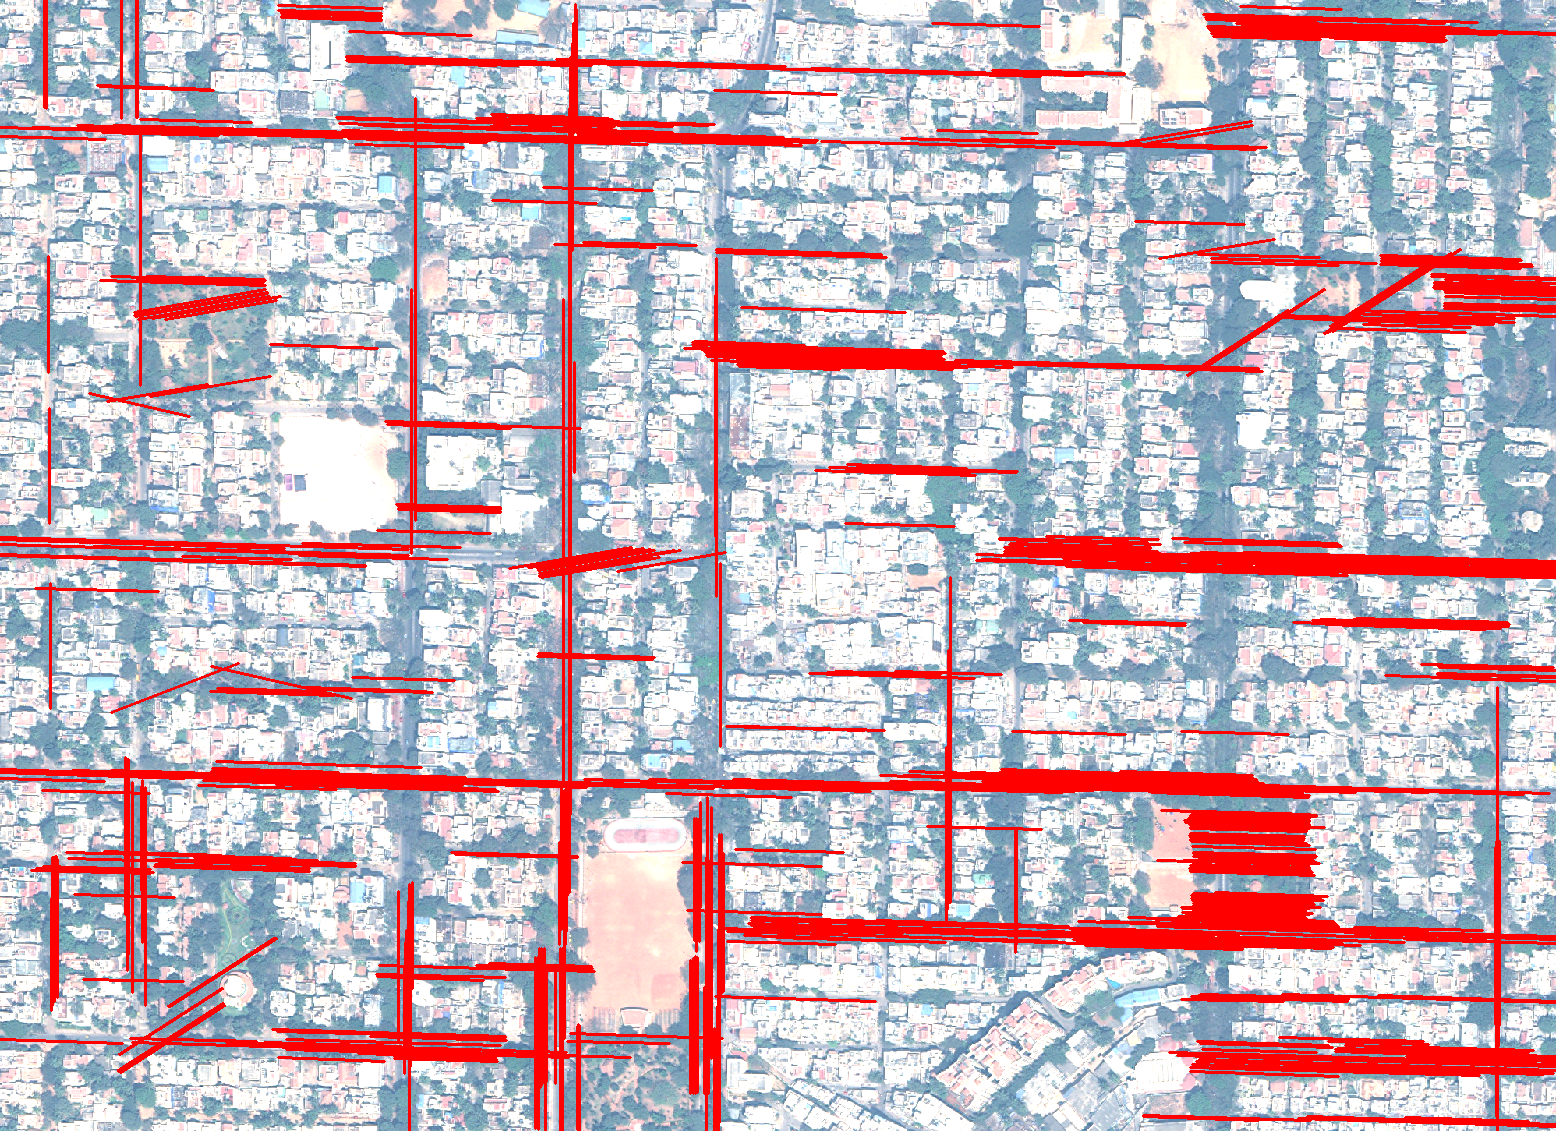
\includegraphics[width=4cm]{images/hough_road_section_8}}&
  \subfloat{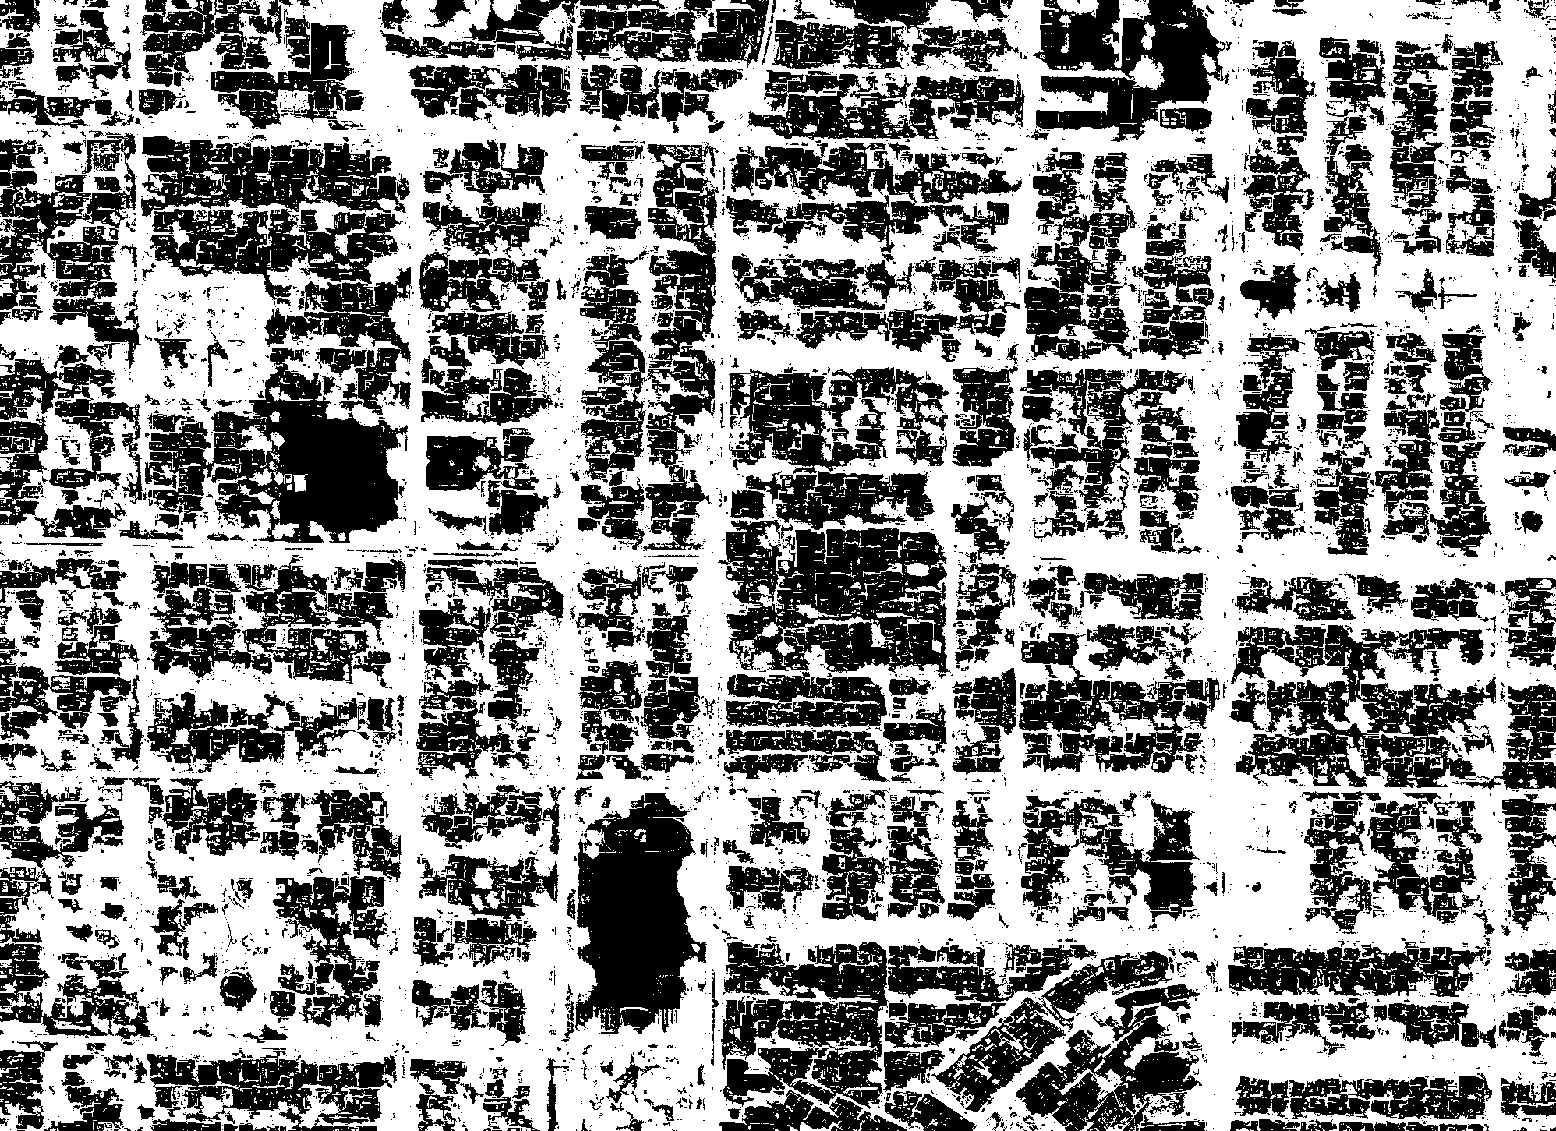
\includegraphics[width=4cm]{images/hough_road_section_8_mask}}
\end{tabular}
\caption{Detected roads using Otsu's thresholding method combined with Hough Transform}
\label{fig:roads_hough}
\end{figure}

This approach was applied in practice in our research. The mask extracted
represented the road network quite accurately. The hough transform resulted in
many correct lines, although there were a lot of duplicates and noise. Although
the noise and duplicates could likely be removed for a large part, we decided
to follow a different method of intersection extraction. 

% TODO: hough transform
% perhaps expand otsu more

% Use opencv canny stuff with hough lines

\subsection{Intersection Convolution}
We designed an new approach to detect intersections using a convolution of
a kernel with its content in the shape of an intersection. Because the kernel
matches the shape of the intersection, the output of the convolution has peaks
in the output image on the positions of the intersections.

This approach has similarites to the use footprints to find the direction of
intersections \cite{hu2007road}. That paper creates certain points, called
seeds, in the image from which the road network expands using road segments.
These roadsegments can be one of a few classes, for example, a straight road,
T junction and cross intersection. The type depends on its surrounding pixels,
which form a footprint that is classified as either one of the classes. In our
research, the detection of crossroad orientation is not important, which is why
less complicated approaches can be used.

\begin{figure}
\[
 \begin{pmatrix}
 0 & 0 & 0 & 1 & 1 & 0 & 0 & 0\\
 0 & 0 & 0 & 1 & 1 & 0 & 0 & 0\\
 0 & 0 & 0 & 1 & 1 & 0 & 0 & 0\\
 1 & 1 & 1 & 1 & 1 & 1 & 1 & 1\\
 1 & 1 & 1 & 1 & 1 & 1 & 1 & 1\\
 0 & 0 & 0 & 1 & 1 & 0 & 0 & 0\\
 0 & 0 & 0 & 1 & 1 & 0 & 0 & 0\\
 0 & 0 & 0 & 1 & 1 & 0 & 0 & 0
 \end{pmatrix}
\] 
\caption{Convolution kernel with a toe width and length of 2 and 3,
respectively}
\label{fig:conv_kernel}
\end{figure}

Before the convolution is performed, the image is first transformed to
grayscale and consequently inverted in color. The grayscale version of the
images have dark roads are bright surroundings. The inversion makes the roads
bright, which will therefore create a peak on convolution instead of create
a dip when no inversion is used.  

The kernel used for the convolution is a n by n matrix, with a cross of ones
filled with zero's, as illustrated in Figure \ref{fig:conv_kernel}. To clarify
some terminology, the toe of an intersection is one of the roads leading to the
intersection. In the case of Figure \ref{fig:conv_kernel}, there are four toes
with a width and length two and three matrix cells, respectively. This kernel
has the optimal activation when it is exactly located on the same shape of the
kernel, thus X intersections. It is therefore important to match the shape of
the kernel to the shape of the intersections in the image. This means that the
width of the toe in the kernel depends on the width of the toe of the
intersections in the image. Therfore, the dimension of the kernel depends on
the image used and the scale of the image.

\begin{figure}
\begin{tabular}{cc}
  \subfloat{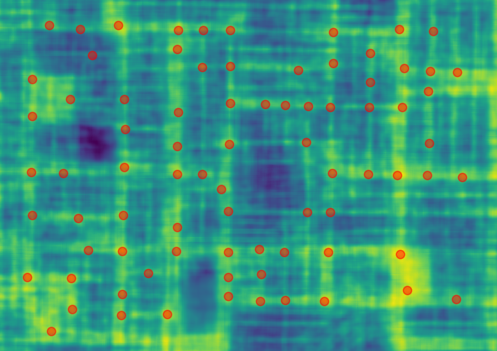
\includegraphics[width=4cm]{images/conv_road_section_8_1}}&
  \subfloat{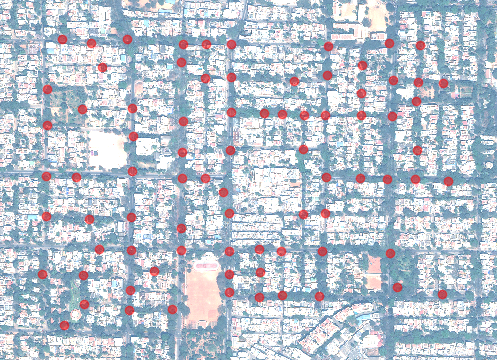
\includegraphics[width=4cm]{images/conv_road_section_8_2}}
\end{tabular}
\caption{Detection of intersections using convolution of a cross shaped kernel.
Left: Heatmap of output of the convolution; Right: Located peaks overlayed on input image}
\label{fig:roads_conv}
\end{figure}

Figure \ref{fig:roads_conv} shows the peaks of the results of the convolution
and the corresponding location of the peaks. The image used was a small section
of the image displayed in Figure \ref{fig:west-bangalore}. It was chosen
because of the regularity of the road network and with 90 degree angles between
the toes of the intersection. Furthermore, the horizontal and vertical roads
run parallel to the edges of the image. Besides, the road network is quite distinct from
the background eventhough it is quite vegetated.

The peaks in the output of the convolution are located using local maxima
detection. This detects, as the name suggests, local maxima in an image. These
are regions that stand out from surrounding area. The location of these maxima
are the red dots displayed over the convolution and the corresponding input
image in Figure \ref{fig:roads_conv}.

A problem to this approach is the orientation of the intersection and roads.
The described kernel only works for intersections which toes are parallel to
the sides of the image. When the intersection are rotated, the kernel does not
match the intersection anymore and will therefore fail to detect it as an
intersection.

Another problem is the need to adjust the parameters to the scale and
resolution of the image. Increasing the scale or resolution of an image will
change the dimensions of the intersection. Because the content of the kernel
must match the intersections in the image pixelwise, the dimensions of the
kernel should change along with change in the image.




%A larger set of images is provided in the appendix.  For the evaluation of this
%intersection detection, we used the 


% what other things also get matched? what goes wrong
